\documentclass[a4paper, 11pt]{article}
\setlength\parindent{0pt}
\usepackage{comment} % enables the use of multi-line comments (\ifx \fi) 
\usepackage{lipsum} %This package just generates Lorem Ipsum filler text. 
\usepackage{fullpage} % changes the margin
\usepackage{amsmath}
\usepackage{mathtools}
\usepackage{graphicx}

\begin{document}
%Header-Make sure you update this information!!!!
\noindent \large\textbf{Homework 02}

\normalsize CS 514 Fall 2018 \hfill Chung Yang 31732286

Algorithms for Data Science \hfill Hao Cheng Cheam 31749564

\rightline{Wenting Wang 31930946}

\rightline{Ye Zhang 31740372}

Prof. Mazumdar \hfill Due Date: Oct 23 2018 \\

\section*{Foundations of Data Science}

\subsection*{7.11}

(1) Example where $x$ minimizing $\sum_{i=1}^n |a_i - x|$ is not unique[figure 1 (a)]:


$x'$ can be any number within [-1, 1] and they all minimize $\sum_{i=1}^n |a_i - x|$, where $a_1 = -1, a_2 = 1$

(2) Example where centroid is different from $x$ that minimize$\sum_{i=1}^n |a_i - x|$ is not unique[figure 1 (b)]:

Data points are $\{-2, -1, 1, 2, 100 \}$

Centroid is $\mu = \frac{-2-1+1+2+100}{5} = 20$

$argmin_x  \sum_{i=1}^n |a_i - x| = 1$ (which is the median of five data points)

The point 1 and 20 are quite far apart.


\begin{figure}[htbp]
	\centering
	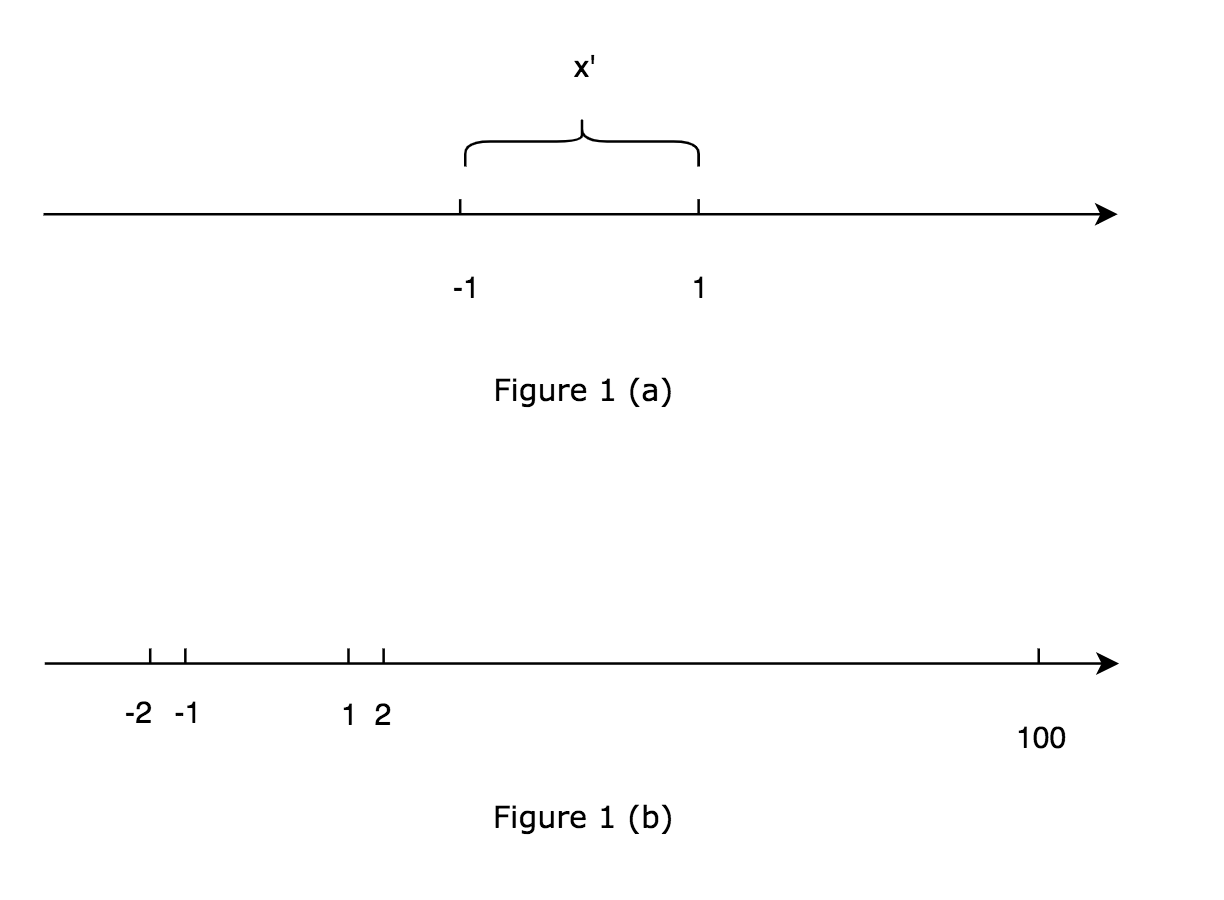
\includegraphics[scale=0.45]{/Users/w/Desktop/CS514/HW2/figure1.png}
\end{figure}

\subsection*{7.12}

Want to show that $\frac{1}{n^2} \sum_{i,j} a_i a_j^T = \frac{1}{n} \sum_{i=1}^n a_i c^T$, $i,j = 1, 2, ..., n$

Known $c = \frac{1}{n} \sum_{i = 1}^n a_i = \frac{1}{n} \sum_{j = 1}^n a_j$

Proof:

$RHS = \frac{1}{n} \sum_{i=1}^n a_i c^T = \frac{1}{n} \sum_{i=1}^n a_i (\frac{1}{n} \sum_{j = 1}^n a_j^T) = \frac{1}{n^2} \sum_{i=1}^n a_i \sum_{j=1}^n a_j^T = \frac{1}{n^2} \sum_{i=1}^n \sum_{J=1}^n a_i a_j^T $

$= \frac{1}{n^2} \sum_{i,j} a_i a_j^T = LHS$

Hence, the average cluster similarity is the same by computing average of all pairs, or average similarity of each point with the centroid of the cluster.

\subsection*{7.17}

The distance of the old and the new centroid is the difference of their weighted average value.

$|\mu (S \cup T) - \mu (S)| = |\frac{\mu (S) |S| + \mu (T) |T|}{|S| + |T|} - \mu (S)| = |\frac{\mu (S) |S| + \mu (T) |T| - \mu (S) (|S| + |T|)}{|S| + |T|}| = \frac{|T|}{|T|+|S|} |\mu (S) - \mu (T)|$.

Thus, the centroid $\mu (S \cup T)$ of $S \cup T$ is at distance at most $\frac{|T|}{|T|+|S|} |\mu (S) - \mu (T)|$ from $\mu (S)$.


\section*{Mining of Massive Datasets}

\subsection*{3.1.1}

For \{1,2,3,4\} and \{2,3,5,7\},  $J = \frac{2}{6} = \frac{1}{3}$. For \{1,2,3,4\} and \{2,4,6\}, $J = \frac{2}{5}$. For \{2,3,5,7\} and \{2,4,6\},  $J = \frac{1}{6}$.

\subsection*{3.1.3}

$$SIM(S,T) = \frac{|S \cap T|}{|S \cup T|} = \frac{k}{2m - k}$$

Suppose $|S \cap T| = k$, where $0 \leq k \leq m$. Then $S$ has $\binom{n}{m}$ choices and $T$ has $\binom{m}{k} \binom{n - m}{m - k}$ choices.

Therefore $P(SIM(S,T) = \frac{k}{2m - k}) = \frac{\binom{m}{k}\binom{n - m}{m - k}}{\binom nm}$

and $E(SIM(S,T)) = \sum_{k=0}^m  \frac{\binom{m}{k}\binom{n - m}{m - k}}{\binom nm} \frac{k}{2m -k}$


\subsection*{3.3.2}

The values of the two hash functions applied to the row numbers are given in the last two columns below

\

\begin{tabular}{c|c|c|c|c|c|c} 
Rows & $S_1$ & $S_2$ & $S_3$ & $S_4$ & $2x + 4 \ mod \ 5$ & $3x - 1 \ mod \ 5$ \\ 
\hline 
0 & 1 & 0 & 0 & 1 & 4 & 4 \\ 
1 & 0 & 0 & 1 & 0 & 1 & 2 \\ 
2 & 0 & 1 & 0 & 1 & 3 & 0 \\ 
3 & 1 & 0 & 1 & 1 & 0 & 3 \\ 
4& 0 & 0 & 1 & 0 & 2 & 1 \\ 
\end{tabular} 

\

The added signature matrix is

\

\begin{tabular}{c|c|c|c|c} 
\ & $S_1$ & $S_2$ & $S_3$ & $S_4$ \\ 
\hline 
$h_1$ & 1 & 3 & 0 & 1  \\ 
$h_2$ & 0 & 2 & 0 & 0 \\
$h_3$ & 0 & 3 & 0 & 0 \\
$h_4$ & 3 & 0 & 1 & 0 \\
\end{tabular} 

\

The calculating process is as follow

\

$\begin{bmatrix}
\infty & \infty & \infty & \infty \\
\infty & \infty & \infty & \infty
\end{bmatrix} \xrightarrow{\text{row(0)}}
\begin{bmatrix}
4 & \infty & \infty & 4 \\
4 & \infty & \infty & 4
\end{bmatrix} \xrightarrow{\text{row(1)}}
\begin{bmatrix}
4 & \infty & 1 & 4 \\
4 & \infty & 2 & 4
\end{bmatrix} \xrightarrow{\text{row(2)}}
\begin{bmatrix}
4 & 3 & 1 & 3 \\
4 & 0 & 2 & 0
\end{bmatrix} \xrightarrow{\text{row(3)}}
\begin{bmatrix}
0 & 3 & 0 & 0 \\
3 & 0 & 2 & 0
\end{bmatrix} \xrightarrow{\text{row(4)}}
\begin{bmatrix}
0 & 3 & 0 & 0 \\
3 & 0 & 1 & 0
\end{bmatrix}
$

\subsection*{3.3.3}

\textbf{(a)} The matrix with hash funstions values is

\

\begin{tabular}{c|c|c|c|c|c|c|c} 
Element & $S_1$ & $S_2$ & $S_3$ & $S_4$ & $2x + 1 \ mod \ 6$ & $3x + 2 \ mod \ 6$ & $5x + 2 \ mod \ 6$ \\ 
\hline 
0 & 0 & 1 & 0 & 1 & 1 & 2 & 2 \\ 
1 & 0 & 1 & 0 & 0 & 3 & 5 & 1 \\ 
2 & 1 & 0 & 0 & 1 & 5 & 2 & 0 \\ 
3 & 0 & 0 & 1 & 0 & 1 & 5 & 5 \\ 
4 & 0 & 0 & 1 & 1 & 3 & 2 & 4 \\ 
5 & 1 & 0 & 0 & 0 & 5 & 5 & 3 \\
\end{tabular} 

\

The signature matrix is

\

\begin{tabular}{c|c|c|c|c} 
\ & $S_1$ & $S_2$ & $S_3$ & $S_4$ \\ 
\hline 
$h_1$ & 5 & 1 & 1 & 1  \\ 
$h_2$ & 2 & 2 & 2 & 2 \\
$h_3$ & 0 & 1 & 4 & 0 \\
\end{tabular} 

\

The calculating process is as follow

\

$\begin{bmatrix}
\infty & \infty & \infty & \infty \\
\infty & \infty & \infty & \infty \\
\infty & \infty & \infty & \infty
\end{bmatrix} \xrightarrow{\text{row(0)}}
\begin{bmatrix}
\infty & 1 & \infty & 1 \\
\infty & 2 & \infty & 2 \\
\infty & 2 & \infty & 2
\end{bmatrix} \xrightarrow{\text{row(1)}}
\begin{bmatrix}
\infty & 1 & \infty & 1 \\
\infty & 2 & \infty & 2 \\
\infty & 1 & \infty & 2
\end{bmatrix} \xrightarrow{\text{row(2)}}
\begin{bmatrix}
5 & 1 & \infty & 1 \\
2 & 2 & \infty & 2 \\
0 & 1 & \infty & 0
\end{bmatrix} \xrightarrow{\text{row(3)}}
\begin{bmatrix}
5 & 1 & 1 & 1 \\
2 & 2 & 5 & 2 \\
0 & 1 & 5 & 0
\end{bmatrix} \xrightarrow{\text{row(4)}}
\begin{bmatrix}
5 & 1 & 1 & 1 \\
2 & 2 & 2 & 2 \\
0 & 1 & 4 & 0
\end{bmatrix} \xrightarrow{\text{row(5)}}
\begin{bmatrix}
5 & 1 & 1 & 1 \\
2 & 2 & 2 & 2 \\
0 & 1 & 4 & 0
\end{bmatrix}
$

\

\textbf{(b)} Only $\{h_3(x) = 5x + 2 \ mod \ 6 \}$ is a true permutation, since there is no collision, i.e. no two rows get the same hash value.

\textbf{(c)} Thematrix of true Jaccard similarities and estimated Jaccard similarities matrix is

\

\begin{tabular}{l|c|c|c|c|c|c} 
Pairs &  $(S_1, S_2)$ & $(S_1, S_3)$ & $(S_1, S_4)$ & $(S_2, S_3)$ & $(S_2, S_4)$ & $(S_3, S_4)$\\ 
\hline
True Jaccard Similarity & 0 & 0 & $\frac{1}{4}$ & 0 & $\frac{1}{4}$ & $\frac{1}{4}$ \\
Estimated Jaccard Similarity & $\frac{1}{3}$ & $\frac{1}{3}$  & $\frac{2}{3}$ & $\frac{2}{3}$ & $\frac{2}{3}$ & $\frac{2}{3}$ \\ 
\end{tabular} 

\subsection*{10.4.1}

\textbf{(a)} The adjacency matrix:

$$A = \begin{bmatrix}
0 &  1 & 1 & 0 & 0 & 0 & 0 & 0 & 0 \\
1 & 0 & 1 & 0 & 0 & 0 & 0 & 1 & 0 \\
1 & 1 & 0 & 1 & 0 & 0 & 0 & 0 & 0 \\
0 & 0 & 1 & 0 & 1 & 1 & 0 & 0 & 0 \\
0 & 0 & 0 & 1 & 0 & 1 & 1 & 0 & 0 \\
0 & 0 & 0 & 1 & 1 & 0 & 0 & 0 & 0 \\
0 & 0 & 0 & 0 & 1 & 0 & 0 & 1 & 1 \\
0 & 1 & 0 & 0 & 0 & 0 & 1 & 0 & 1 \\
0 & 0 & 0 & 0 & 0 & 0 & 1 & 1 & 0
\end{bmatrix}$$

\textbf{(b)} The degree matrix:

$$ D =  \begin{bmatrix}
2 & 0 & 0 & 0 & 0 & 0 & 0 & 0 & 0 \\
0 & 3 & 0 & 0 & 0 & 0 & 0 & 0 & 0 \\
0 & 0 & 3 & 0 & 0 & 0 & 0 & 0 & 0 \\
0 & 0 & 0 & 3 & 0 & 0 & 0 & 0 & 0 \\
0 & 0 & 0 & 0 & 3 & 0 & 0 & 0 & 0 \\
0 & 0 & 0 & 0 & 0 & 2 & 0 & 0 & 0 \\
0 & 0 & 0 & 0 & 0 & 0 & 3 & 0 & 0 \\
0 & 0 & 0 & 0 & 0 & 0 & 0 & 3 & 0 \\
0 & 0 & 0 & 0 & 0 & 0 & 0 & 0 & 2 
\end{bmatrix}  $$

\textbf{(c)} The Laplacian matrix

$$L = D - A = \begin{bmatrix}
2 &  -1 & -1 & 0 & 0 & 0 & 0 & 0 & 0 \\
-1 & 3 & -1 & 0 & 0 & 0 & 0 & -1 & 0 \\
-1 & -1 & 3 & -1 & 0 & 0 & 0 & 0 & 0 \\
0 & 0 & -1 & 3 & -1 & -1 & 0 & 0 & 0 \\
0 & 0 & 0 & -1 & 3 & -1 & -1 & 0 & 0 \\
0 & 0 & 0 & -1 & -1 & 2 & 0 & 0 & 0 \\
0 & 0 & 0 & 0 & -1 & 0 & 3 & -1 & -1 \\
0 & -1 & 0 & 0 & 0 & 0 & -1 & 3 & -1 \\
0 & 0 & 0 & 0 & 0 & 0 & -1 & -1 & 2
\end{bmatrix}$$


\subsection*{10.4.2} 

The code file: q10\_4\_2.py

For the Laplacian matrix above, implement eigendecomposition, obtain the second-smallest eigenvalue is  0.69722436226800433, the corresponding vector is  [-0.15728598, -0.16666667, 0.29389153, -0.33333333, 0.28305594, -0.40824829,  0.50834187,  0.00210742, -0.48643259].

The second eigenvector has four positive and five negative components, which suggests that one group should be \{C, E, G, H\}, the nodes with positive components; and the other group should be \{A, B, D, F, I\}, the nodes with positive components. 

The partition is however unbalanced, even by changing the threshold. Check the eigendecomposition again, the third-smallest eigenvalue is 0.69722436226800577, which is very close to the second-smallest eigenvalue, the corresponding vector is [-0.36219431,  0.33333333, -0.38287473, -0.33333333  0.10413675, -0.40824829, -0.3923125,  0.23920786, -0.07430338]

Thus consider the second and the third vectors together, the new partition is \{A, D, F, I\} (negative values in both vectors), \{B\} (negative in the second, positive in the third vector), \{C, G\} (positive in the second, negative in the third vector), \{E, H\} (positive in both vectors).

The new partition is either balanced for the graph, further eigenvalues and vectors are ought to be considered.
  
\section*{Coding Assignment}

\subsection*{7.4}

The code file q7\_14.py

\section*{Attachments}

q7\_14.py, q10\_4\_2.py


\end{document}